% ============================================================================
%  Chapter 5 — Sprint 2: Policy Expansion and Threshold Configuration
% ============================================================================

\chapter{Sprint 2: Policy Expansion and Threshold Configuration}
\label{chap:sprint2}

\section{Introduction}

The second sprint turned the microservice from a proof-of-concept with twelve policies into a real security scanning platform with 103~policies across 15~categories. We also added a configurable severity threshold and a diff-only scanning mode, making the system much more flexible and practical for real-world use.


\section{Sprint Objectives}

\begin{enumerate}[leftmargin=1.5cm]
  \item Expand the policy library from 12 to 103 policies, covering all major AWS services, Docker, Kubernetes, Azure, and GCP.
  \item Add a configurable severity threshold so users can control which violations cause a BLOCK.
  \item Implement diff-only scanning to evaluate only changed lines from a unified diff.
  \item Make sure all existing tests still pass.
\end{enumerate}


\section{Sprint Backlog}

\begin{table}[H]
\centering
\begin{tabularx}{\textwidth}{|c|X|c|c|}
\hline
\textbf{ID} & \textbf{Task} & \textbf{Story} & \textbf{Status} \\
\hline
T-13 & Implement AWS S3 extended policies (versioning, MFA delete, lifecycle, public ACL block). & US-08 & Done \\
\hline
T-14 & Implement AWS EC2 policies (IMDSv2, public IP, key pair, EBS encryption, monitoring, termination protection, user data secrets). & US-08 & Done \\
\hline
T-15 & Implement AWS RDS policies (Multi-AZ, backup retention, deletion protection, IAM auth, minor version upgrade, public subnet, logging). & US-08 & Done \\
\hline
T-16 & Implement AWS IAM policies (MFA, admin access, password policy, root usage, key rotation, cross-account, unused credentials). & US-08 & Done \\
\hline
T-17 & Implement AWS VPC policies (flow logs, default SG, NACLs, peering, endpoint, IPv6). & US-08 & Done \\
\hline
T-18 & Implement extended Docker policies (ADD instruction, secrets in ENV, COPY --chown, healthcheck, latest tag). & US-09 & Done \\
\hline
T-19 & Implement extended Kubernetes policies (privilege escalation, root user, read-only FS, capabilities, liveness/readiness probes, namespace, service account, image pull). & US-09 & Done \\
\hline
T-20 & Implement remaining categories (CloudTrail, ELB/WAF, Terraform general, EKS/Lambda/ECS, messaging, ECR/CloudFront, Azure/GCP). & US-08 & Done \\
\hline
T-21 & Implement configurable \texttt{block\_threshold} parameter. & US-10 & Done \\
\hline
T-22 & Implement diff-only scanning mode. & US-11 & Done \\
\hline
\end{tabularx}
\caption{Sprint 2 backlog.}
\label{tab:s2-backlog}
\end{table}


\section{Use Case Refinement}

\subsection{Use Case: Analyze with Configurable Threshold}

\begin{table}[H]
\centering
\begin{tabularx}{\textwidth}{|l|X|}
\hline
\textbf{Use Case} & Analyze with Configurable Threshold \\
\hline
\textbf{Actor} & Security Officer \\
\hline
\textbf{Precondition} & The policy service is running; the actor knows the available severity levels. \\
\hline
\textbf{Postcondition} & Only violations at or above the chosen threshold cause a BLOCK. \\
\hline
\textbf{Nominal Scenario} &
  \begin{enumerate}[leftmargin=0.8cm, nosep]
    \item The actor sends a POST to \texttt{/analyze} with \texttt{block\_threshold} set to \texttt{HIGH}.
    \item The engine runs all policies and collects every violation.
    \item Only violations with severity $\geq$ HIGH are treated as blocking.
    \item If there are blocking violations, the decision is BLOCK; otherwise ALLOW.
    \item LOW and MEDIUM violations are still reported but do not cause blocking.
  \end{enumerate} \\
\hline
\end{tabularx}
\caption{Textual description --- ``Analyze with Configurable Threshold'' use case.}
\label{tab:uc-threshold}
\end{table}


\section{Sequence Diagram}

\begin{figure}[H]
\centering
\begin{tikzpicture}[
    participant/.style = {
        draw, thick, rectangle, rounded corners=2pt,
        minimum width=1.8cm, minimum height=0.6cm,
        align=center, font=\scriptsize\bfseries,
        fill=#1
    },
    msg/.style = {-{Stealth[length=4pt]}, thick},
    ret/.style = {-{Stealth[length=4pt]}, thick, dashed}
]

% Participants
\node[participant=gray!15] (client) at (0, 0) {Client};
\node[participant=blue!15] (api) at (4, 0) {API};
\node[participant=red!15] (engine) at (8, 0) {PolicyEngine};
\node[participant=orange!15] (filter) at (12, 0) {Threshold\\Filter};

% Lifelines
\foreach \n in {client, api, engine, filter}
    \draw[dashed, thin, gray] (\n.south) -- ++(0, -7.5);

% Messages
\draw[msg] (0, -1) -- node[above, font=\tiny] {POST /analyze \{threshold: HIGH\}} (4, -1);
\draw[msg] (4, -1.8) -- node[above, font=\tiny] {analyze(code, threshold)} (8, -1.8);

% Loop
\draw[thick, rounded corners=2pt] (7, -2.3) rectangle (9.5, -3.3);
\node[font=\tiny, anchor=north west] at (7.1, -2.35) {loop [103 policies]};
\node[font=\tiny] at (8.25, -2.85) {policy.check()};

\draw[msg] (8, -3.8) -- node[above, font=\tiny] {filter(violations, HIGH)} (12, -3.8);

% Filter decision
\draw[thick, rounded corners=2pt] (10.5, -4.3) rectangle (13.5, -5.5);
\node[font=\tiny, anchor=north west] at (10.6, -4.35) {alt};
\node[font=\tiny] at (12, -4.75) {sev $\geq$ HIGH $\rightarrow$ blocking};
\node[font=\tiny] at (12, -5.2) {sev $<$ HIGH $\rightarrow$ non-blocking};

\draw[ret] (12, -5.8) -- node[above, font=\tiny] {blocking\_violations} (8, -5.8);
\draw[ret] (8, -6.4) -- node[above, font=\tiny] {decision + all violations} (4, -6.4);
\draw[ret] (4, -7) -- node[above, font=\tiny] {AnalyzeResponse (JSON)} (0, -7);

\end{tikzpicture}
\caption{Sprint 2 sequence diagram: threshold filtering separates blocking from non-blocking violations.}
\label{fig:s2-sequence}
\end{figure}


\section{Realization}

\subsection{Policy Categories and Distribution}

The 103~policies are organized across 15~categories. Table~\ref{tab:policy-categories} shows how they are distributed.

\begin{table}[H]
\centering
\begin{tabular}{|c|l|c|c|}
\hline
\textbf{\#} & \textbf{Category} & \textbf{Policies} & \textbf{Severity Range} \\
\hline
1  & Core Policies (AWS S3, EC2, RDS, Docker, K8s) & 12 & CRITICAL--LOW \\
\hline
2  & AWS S3 Extended                               &  4 & HIGH--LOW \\
\hline
3  & AWS EC2 / Compute                             &  7 & CRITICAL--LOW \\
\hline
4  & AWS RDS / Database                            &  7 & HIGH--MEDIUM \\
\hline
5  & AWS IAM / Identity                            &  7 & CRITICAL--MEDIUM \\
\hline
6  & AWS VPC / Networking                          &  6 & HIGH--MEDIUM \\
\hline
7  & Docker Extended                               &  8 & HIGH--LOW \\
\hline
8  & Kubernetes Extended                           & 12 & HIGH--LOW \\
\hline
9  & AWS CloudTrail / Audit \& Compliance           &  8 & HIGH--MEDIUM \\
\hline
10 & ELB / ALB / WAF / Route53                     &  7 & HIGH--MEDIUM \\
\hline
11 & Terraform General                             &  5 & HIGH--LOW \\
\hline
12 & EKS / Lambda / ECS                            &  7 & HIGH--MEDIUM \\
\hline
13 & Messaging / Cache / DynamoDB                  &  5 & HIGH--MEDIUM \\
\hline
14 & ECR / Secrets Manager / CloudFront            &  5 & HIGH--MEDIUM \\
\hline
15 & Azure / GCP Bonus                             &  3 & CRITICAL--HIGH \\
\hline
   & \textbf{Total}                                & \textbf{103} & \\
\hline
\end{tabular}
\caption{Distribution of 103 security policies across 15 categories.}
\label{tab:policy-categories}
\end{table}

\begin{figure}[H]
\centering
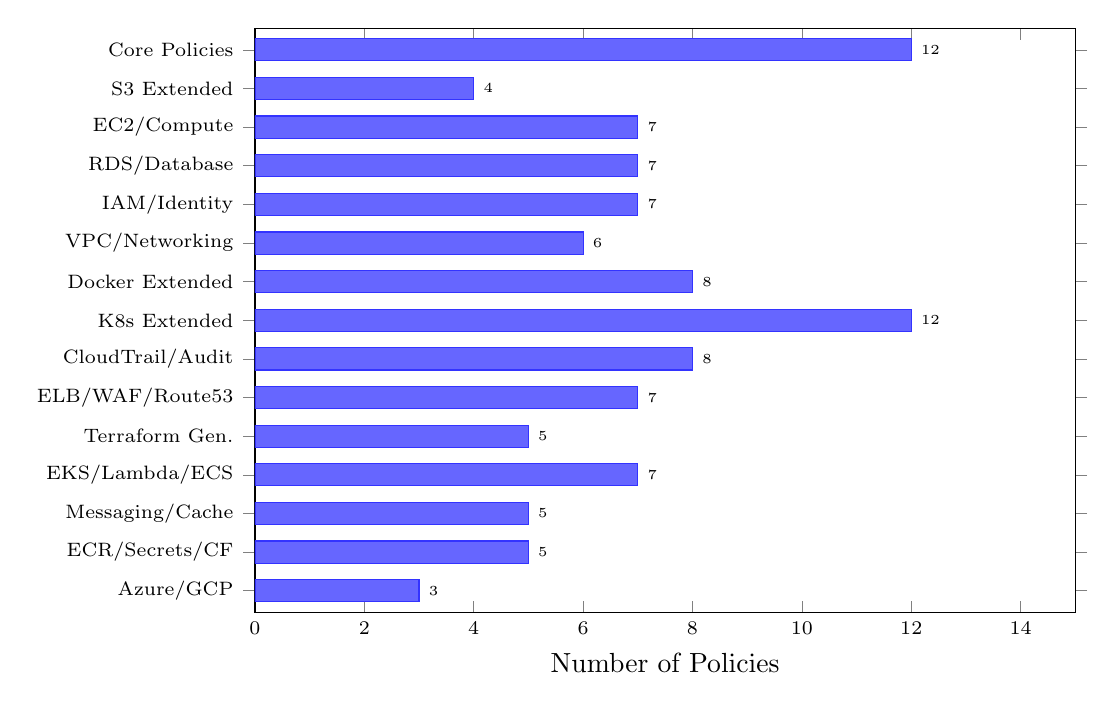
\begin{tikzpicture}
\begin{axis}[
    xbar,
    width=12cm, height=9cm,
    xlabel={Number of Policies},
    symbolic y coords={
        {Azure/GCP},
        {ECR/Secrets/CF},
        {Messaging/Cache},
        {EKS/Lambda/ECS},
        {Terraform Gen.},
        {ELB/WAF/Route53},
        {CloudTrail/Audit},
        {K8s Extended},
        {Docker Extended},
        {VPC/Networking},
        {IAM/Identity},
        {RDS/Database},
        {EC2/Compute},
        {S3 Extended},
        {Core Policies}
    },
    ytick=data,
    y tick label style={font=\scriptsize},
    x tick label style={font=\scriptsize},
    nodes near coords,
    nodes near coords align={horizontal},
    every node near coord/.append style={font=\tiny},
    bar width=8pt,
    xmin=0, xmax=15,
    enlarge y limits=0.04,
]
\addplot[fill=blue!60, draw=blue!80] coordinates {
    (12,{Core Policies})
    (4,{S3 Extended})
    (7,{EC2/Compute})
    (7,{RDS/Database})
    (7,{IAM/Identity})
    (6,{VPC/Networking})
    (8,{Docker Extended})
    (12,{K8s Extended})
    (8,{CloudTrail/Audit})
    (7,{ELB/WAF/Route53})
    (5,{Terraform Gen.})
    (7,{EKS/Lambda/ECS})
    (5,{Messaging/Cache})
    (5,{ECR/Secrets/CF})
    (3,{Azure/GCP})
};
\end{axis}
\end{tikzpicture}
\caption{Distribution of 103 security policies across the 15 categories.}
\label{fig:policy-distribution}
\end{figure}

\subsection{Severity Threshold Mechanism}

The threshold mechanism gives users fine-grained control over what triggers a BLOCK. The severity levels are ranked as follows:

\begin{center}
\texttt{CRITICAL (4) > HIGH (3) > MEDIUM (2) > LOW (1) > INFO (0)}
\end{center}

When a user sets \texttt{block\_threshold} to \texttt{HIGH}, only violations rated HIGH or CRITICAL can cause a BLOCK. Lower-severity violations are still included in the response, but they are marked as non-blocking.

\begin{lstlisting}[language=Python, caption={Severity threshold filtering logic.}, label={lst:threshold}]
SEV_ORDER = {'CRITICAL': 4, 'HIGH': 3, 'MEDIUM': 2, 'LOW': 1, 'INFO': 0}

# In PolicyEngine.analyze():
threshold_level = SEV_ORDER.get(block_threshold.upper(), 1)
blocking_violations = [
    v for v in all_violations
    if SEV_ORDER.get(v.severity.value, 0) >= threshold_level
]
allow = len(blocking_violations) == 0
\end{lstlisting}

This feature is important for real-world adoption. A team that is just starting to use the service can begin with a CRITICAL-only threshold and gradually lower it as they fix existing violations.

\subsection{Diff-Only Scanning Mode}

The diff-only mode solves a common problem: when a team first adds the scanner to their CI/CD pipeline, the existing codebase might have hundreds of old violations. Scanning only the changed lines lets teams enforce policies on new code without being buried under issues from the past.

\begin{lstlisting}[language=Python, caption={Diff-only filtering in the policy engine.}, label={lst:diff-only}]
def parse_diff_lines(diff: str) -> set:
    """Extract line numbers added/changed in a unified diff."""
    changed_lines = set()
    current_line = 0
    for line in diff.splitlines():
        if line.startswith('@@'):
            match = re.search(r'\+(\d+)', line)
            if match:
                current_line = int(match.group(1)) - 1
        elif line.startswith('+') and not line.startswith('+++'):
            current_line += 1
            changed_lines.add(current_line)
        elif not line.startswith('-'):
            current_line += 1
    return changed_lines
\end{lstlisting}

\subsection{Policy Implementation Examples}

\subsubsection{EC2 IMDSv2 Enforcement}

This HIGH-severity policy detects EC2 instances that do not enforce IMDSv2, which is important for preventing SSRF attacks that exploit the Instance Metadata Service:

\begin{lstlisting}[language=Python, caption={EC2 IMDSv2 policy (excerpt).}, label={lst:imdsv2}]
class EC2IMDSv1EnabledPolicy(BasePolicy):
    def check(self, code):
        violations = []
        for instance in code.find_resources_by_type("aws_instance"):
            metadata = instance.get_attribute("metadata_options", {})
            http_tokens = metadata.get("http_tokens", "optional")
            if http_tokens != "required":
                violations.append(PolicyViolation(
                    rule_id="EC2_IMDSV1_ENABLED",
                    severity=PolicySeverity.HIGH,
                    message=f"EC2 '{instance.resource_name}' allows IMDSv1",
                    recommendation="Set http_tokens = 'required' in metadata_options"
                ))
        return violations
\end{lstlisting}

\subsubsection{Kubernetes Privilege Escalation}

This HIGH-severity policy catches containers that allow privilege escalation, a common Kubernetes misconfiguration that can lead to container breakout attacks:

\begin{lstlisting}[language=Python, caption={K8s privilege escalation policy (excerpt).}, label={lst:k8s-privesc}]
class K8sAllowPrivilegeEscalationPolicy(BasePolicy):
    def check(self, code):
        violations = []
        if code.code_type != "kubernetes":
            return violations
        for resource in code.resources:
            if "container" in resource.resource_type:
                sec_ctx = resource.get_attribute("securityContext", {})
                if sec_ctx.get("allowPrivilegeEscalation", True):
                    violations.append(PolicyViolation(
                        rule_id="K8S_ALLOW_PRIVILEGE_ESCALATION",
                        severity=PolicySeverity.HIGH,
                        message=f"Container '{resource.resource_name}' allows privilege escalation",
                        recommendation="Set allowPrivilegeEscalation: false"
                    ))
        return violations
\end{lstlisting}


\section{Tests}

All seven existing tests continued to pass after adding the new policies, which confirms that the expansion did not break anything. The threshold behavior was validated through the existing safe code test:

\begin{lstlisting}[language=Python, caption={Threshold validation test.}, label={lst:threshold-test}]
def test_analyze_safe_code():
    request_data = {
        "code_type": "terraform",
        "content": 'resource "aws_s3_bucket" "safe" { acl = "private" }',
        "block_threshold": "CRITICAL"
    }
    response = client.post("/analyze", json=request_data)
    data = response.json()
    assert data["decision"] == "ALLOW"
\end{lstlisting}


\section{Interfaces}

\figplaceholder{Server startup: 103 policies loaded}{policies_loaded}
\figplaceholder{Threshold comparison: ALLOW vs BLOCK}{threshold_comparison}


\section{Conclusion}

Sprint~2 grew the microservice from 12 to 103~security policies across 15~categories, added the configurable severity threshold for gradual adoption, and introduced diff-only scanning for teams with existing codebases. Despite an 8.5$\times$ increase in the number of policies, the average response time stayed under 50\,ms, showing that the layered architecture scales well. The next sprint builds the user-facing features: the web dashboard, auto-fix engine, and compliance reports.
